%%%%%%%%%%%%%%%%%%%%%%%%%%%%%%%%%%%%%%%%%%%%%%%%%%%%%%%%%%%%%%%%%%%%%%%%%%%%%%%%%%%%%
% PACOTES                                                                           %
%%%%%%%%%%%%%%%%%%%%%%%%%%%%%%%%%%%%%%%%%%%%%%%%%%%%%%%%%%%%%%%%%%%%%%%%%%%%%%%%%%%%%
\documentclass[a4paper,12pt]{article}

%-----------------------------------------------------------------------------------%
% LAYOUT DA PÁGINA                                                                  %
%-----------------------------------------------------------------------------------%
\usepackage[top=3cm, bottom=3cm, left=2.5cm, right=2.5cm]{geometry}
%\usepackage{fancyhdr} % Permite controlar como são exibidos os cabeçalhos

%-----------------------------------------------------------------------------------%
% FORMATAÇÃO DO TEXTO                                                               %
%-----------------------------------------------------------------------------------%
%\usepackage{setspace} % Permite definir o espaçamento entre linhas

%-----------------------------------------------------------------------------------%
% PACOTES DE IMAGENS                                                                %
%-----------------------------------------------------------------------------------%
\usepackage[pdftex]{graphicx}
%\usepackage[pstarrows]{pict2e} % Amplia as funcionalidades do ambiente picture

%-----------------------------------------------------------------------------------%
% PACOTES DE TABELAS                                                                %
%-----------------------------------------------------------------------------------%
\usepackage{array} % Facilita a formatação de tabelas
%\usepackage{multirow} % Permite criar células que ocupam várias linhas em uma tabela
\usepackage{longtable} % Permite criar tabelas que quebram de página

%-----------------------------------------------------------------------------------%
% PACOTES MATEMÁTICOS DE BASE                                                       %
%-----------------------------------------------------------------------------------%
\usepackage{amsfonts,amstext,amscd,bezier,amsthm,amssymb}
\usepackage[centertags]{amsmath}

%-----------------------------------------------------------------------------------%
% PACOTES DE SÍMBOLOS MATEMÁTICOS                                                   %
%-----------------------------------------------------------------------------------%
%\usepackage{mathtools} % Símbolos matemáticos extras. (ex.: \xrightharpoon)
%\usepackage[integrals]{wasysym} % Muda o estilo das integrais, além de outros
%                                 símbolos extras
%\usepackage[nice]{nicefrac} % Permite o uso de frações "melhores". Usar \nicefrac{}{}

%-----------------------------------------------------------------------------------%
% PACOTES DE FONTES MATEMÁTICAS                                                     %
%-----------------------------------------------------------------------------------%
%\usepackage{mathbbol} % Quase todos os símbolos com \mathbb
%\usepackage{bbm} % Extensão dos símbolos de \mathbb. Usar comando \mathbbm
%\usepackage{calrsfs} % Muda o estilo de \mathcal
%\usepackage[mathcal]{euscript} % Muda o estilo de \mathcal

%-----------------------------------------------------------------------------------%
% PACOTES DE CODIFICAÇÃO DE FONTES                                                  %
%-----------------------------------------------------------------------------------%
\usepackage[utf8]{inputenc} % Permite o uso de caracteres ISO 8859-1, incluindo os
%                               caracteres acentuados diretamente.
\usepackage[T1]{fontenc} % Uso de fontes T1, necessário para tratar caracteres
%                          acentuados como um único bloco.

%-----------------------------------------------------------------------------------%
% PACOTES DE LÍNGUAS                                                                %
%-----------------------------------------------------------------------------------%
\usepackage[francais]{babel} % Seleciona a língua do documento, definindo nomes de
%                              seções, nome do índice, da bibliografia, etc. Em caso
%                              de documento com mais de uma língua, a padrão é a
%                              última.
\NoAutoSpaceBeforeFDP % Utilizar em francês se quiser evitar espaços antes de :

%-----------------------------------------------------------------------------------%
% PACOTES DE BIBLIOGRAFIA                                                           %
%-----------------------------------------------------------------------------------%
%\usepackage{babelbib} % Permite definir a língua das entradas da bibliografia. Usar
%                       [fixlanguage] para uma mesma língua para todas as entradas e
%                       \selectbiblanguage{} para definir a língua. Um estilo compa-
%                       tível com babelbib deve ser usado (ex: babplain)
\usepackage{cite} % Organiza os elementos citados dentro de um mesmo \cite.

%-----------------------------------------------------------------------------------%
% PACOTES DE FONTES                                                                 %
%-----------------------------------------------------------------------------------%
% Computer Modern (fonte padrão)                                                    %
% - - - - - - - - - - - - - - - - - - - - - - - - - - - - - - - - - - - - - - - - - %
%\usepackage{ae} % A usar com a fonte padrão do LaTeX quando forem gerados PDFs, para
%                 corrigir erros de visualização

% Computer Modern Bright (sans serif)                                               %
% - - - - - - - - - - - - - - - - - - - - - - - - - - - - - - - - - - - - - - - - - %
%\usepackage{cmbright}

% Times New Roman                                                                   %
% - - - - - - - - - - - - - - - - - - - - - - - - - - - - - - - - - - - - - - - - - %
%\usepackage{mathptmx} % Muda texto e modo matemático
%\usepackage{times} % Apenas texto, não muda modo matemático

% Arial                                                                             %
% - - - - - - - - - - - - - - - - - - - - - - - - - - - - - - - - - - - - - - - - - %
%\usepackage[scaled]{uarial} % Arial como fonte sans serif padrão

% Palatino                                                                          %
% - - - - - - - - - - - - - - - - - - - - - - - - - - - - - - - - - - - - - - - - - %
%\usepackage{mathpazo} % Muda texto e modo matemático
%\usepackage{palatino} % Apenas texto, não muda modo matemático

% Concrete                                                                          %
% - - - - - - - - - - - - - - - - - - - - - - - - - - - - - - - - - - - - - - - - - %
%\usepackage{ccfonts} % Texto: Concrete; Matemático: Concrete Math
%\usepackage{ccfonts, eulervm} % Texto: Concrete; Matemático: Euler

% Iwona                                                                             %
% - - - - - - - - - - - - - - - - - - - - - - - - - - - - - - - - - - - - - - - - - %
%\usepackage[math]{iwona} % Texto e modo matemático: Iwona

% Kurier                                                                            %
% - - - - - - - - - - - - - - - - - - - - - - - - - - - - - - - - - - - - - - - - - %
%\usepackage[math]{kurier} % Texto e modo matemático: Kurier

% Antykwa Póltawskiego                                                              %
% - - - - - - - - - - - - - - - - - - - - - - - - - - - - - - - - - - - - - - - - - %
%\usepackage{antpolt} % Texto: Antykwa Póltawskiego; Matemático: nenhum
                     % Usar fontenc = QX ou OT4

% Utopia                                                                            %
% - - - - - - - - - - - - - - - - - - - - - - - - - - - - - - - - - - - - - - - - - %                     
%\usepackage{fourier} % Texto: Utopia; Matemático: Fourier

% KP Serif                                                                          %
% - - - - - - - - - - - - - - - - - - - - - - - - - - - - - - - - - - - - - - - - - %
\usepackage{kpfonts}

%-----------------------------------------------------------------------------------%
% CORES                                                                             %
%-----------------------------------------------------------------------------------%
\usepackage{color}
\definecolor{darkgreen}{rgb}{0,0.5,0}
\definecolor{darkmagenta}{rgb}{0.5,0,0.5}
\definecolor{darkgray}{rgb}{0.5,0.5,0.5}
\definecolor{darkblue}{rgb}{0.2,0.2,0.4}
\definecolor{darkred}{rgb}{0.6,0.15,0.15}
\definecolor{gray}{rgb}{0.65,0.65,0.65}
\definecolor{lightgray}{rgb}{0.8,0.8,0.8}
\definecolor{lightblue}{rgb}{0.5,0.5,1}
\definecolor{lightgreen}{rgb}{0.5,1,0.5}
\definecolor{deadred}{rgb}{0.7, 0.2, 0.2}
\definecolor{deadblue}{rgb}{0.2, 0.2, 0.7}

%-----------------------------------------------------------------------------------%
% PACOTES DIVERSOS                                                                  %
%-----------------------------------------------------------------------------------%
\usepackage{icomma} % Permite uso de vírgula como separador decimal
\usepackage{url} % Pacote para não ter problemas com URLs. Usar \url{}
%\usepackage{randtext} % Troca a ordem de letras de uma frase (útil com e-mails em
                      % PDFs a serem publicados on-line.
\usepackage[hidelinks]{hyperref}
%\usepackage{showkeys} % Para mostrar o nome dos labels
\usepackage{enumitem} % Facilita o uso de listas, inclusive referências a itens de
                      % listas.
%\usepackage[absolute]{textpos} % Posição absoluta de texto na página
%\usepackage{pdfpages} % Permite incluir documentos em PDF no arquivo
%\usepackage{refcheck} % Verifica as referências procurando por
%                      % labels não usados ou equações numeradas sem labels.
%                      % Verificar o arquivo .log e procurar por RefCheck.

%%%%%%%%%%%%%%%%%%%%%%%%%%%%%%%%%%%%%%%%%%%%%%%%%%%%%%%%%%%%%%%%%%%%%%%%%%%%%%%%%%%%%
% CONFIGURAÇÕES                                                                     %
%%%%%%%%%%%%%%%%%%%%%%%%%%%%%%%%%%%%%%%%%%%%%%%%%%%%%%%%%%%%%%%%%%%%%%%%%%%%%%%%%%%%%

%-----------------------------------------------------------------------------------%
% FORMATAÇÃO DO TEXTO                                                               %
%-----------------------------------------------------------------------------------%
%\onehalfspacing % Espaçamento 1 1/2 (definido no pacote setspace)

%-----------------------------------------------------------------------------------%
% DEFINIÇÃO DE AMBIENTES MATEMÁTICOS                                                %
%-----------------------------------------------------------------------------------%
%\theoremstyle{plain}
%\newtheorem{theo}{Teorema}[section]
%\newtheorem{lemm}[theo]{Lema}
%\newtheorem{coro}[theo]{Corolário}
%\newtheorem{prop}[theo]{Proposição}
%\theoremstyle{definition}
%\newtheorem{defi}[theo]{Definição}
%\newtheorem{remq}[theo]{Observação}
%%\newtheorem{expl}[theo]{Exemplo}
%\newenvironment{expl}%
%  {\refstepcounter{theo}%
%    \begin{list}{}{%
%    \setlength{\topsep}{0pt}%
%    \setlength{\leftmargin}{\parindent}%
%    \setlength{\rightmargin}{0pt}%
%    \setlength{\listparindent}{\parindent}%
%    \setlength{\itemindent}{0pt}%
%    \setlength{\parsep}{\parskip}}%
%    \item[]{\bf Exemplo \thetheo. }}%
%  {\hspace*{\fill} $\square$ \end{list} \medskip}
%\newenvironment{solu}%
%  {\noindent {\bf Solução. }\small}%
%  {\hspace*{\fill} $\square$ \normalsize \medskip}
%\newenvironment{dems}[1][Demonstração]%
%  {\begin{list}{}{%
%    \setlength{\topsep}{0pt}%
%    \setlength{\leftmargin}{\parindent}%
%    \setlength{\rightmargin}{0pt}%
%    \setlength{\listparindent}{\parindent}%
%    \setlength{\itemindent}{0pt}%
%    \setlength{\parsep}{\parskip}}%
%    \item[]{\bf #1. }}%
%  {\hspace*{\fill} $\blacksquare$ \end{list} \medskip}


%-----------------------------------------------------------------------------------%
% DEFINIÇÃO DE COMANDOS MATEMÁTICOS                                                 %
%-----------------------------------------------------------------------------------%
%\newcommand*\diff{\mathop{}\!\mathrm{d}}

%\newcommand{\norm}[1]{\left\lVert #1\right\lVert} % Norma
%\newcommand{\abs}[1]{\left\lvert #1\right \rvert} % Valor absoluto
%\newcommand{\floor}[1]{\left\lfloor #1 \right\rfloor} % Arredondar para baixo
%\newcommand{\ceil}[1]{\left\lceil #1 \right\rceil} % Arredondar para cima


%-----------------------------------------------------------------------------------%
% NUMERAÇÃO DE ELEMENTOS                                                            %
%-----------------------------------------------------------------------------------%
%\numberwithin{table}{section}
%\numberwithin{table}{subsection}
%\numberwithin{figure}{section}
%\numberwithin{figure}{subsection}
\numberwithin{equation}{section}
%\numberwithin{equation}{subsection}
%\numberwithin{theo}{chapter}
%\numberwithin{theo}{subsection}

%%%%%%%%%%%%%%%%%%%%%%%%%%%%%%%%%%%%%%%%%%%%%%%%%%%%%%%%%%%%%%%%%%%%%%%%%%%%%%%%%%%%%
% ESTRUTURA DO DOCUMENTO                                                            %
%%%%%%%%%%%%%%%%%%%%%%%%%%%%%%%%%%%%%%%%%%%%%%%%%%%%%%%%%%%%%%%%%%%%%%%%%%%%%%%%%%%%%
\begin{document}

\title{2I006 \\ Mini-Projet : Gestion d'une bibliothèque}
\author{Ariana Carnielli et Lisa Kacel}
\date{}

\maketitle

\section*{Question 3.1}

La Table \ref{TabQues31} présente les temps de calcul en millisecondes pour réaliser la recherche d'un ouvrage par son numéro ou son titre et la recherche de tous les ouvrages d'un même auteur. Cette simulation a été faite en chargeant toute la bibliothèque du fichier donné (100 000 livres), et on a choisi la taille de la table de hachage comme la moitié de la quantité de livres dans la bibliothèque, soit $m = 50 000$. À chaque recherche, nous avons cherché une donnée non présente dans la bibliothèque pour tester le pire des cas. Chaque recherche a été répétée 100 000 fois.

\begin{table}[ht]
\centering
\begin{tabular}{c|ccc}
\hline\hline
& Numéro & Titre & Auteur \tabularnewline
\hline
Liste chainée & 0,86 & 0,85 & 0,84 \tabularnewline
Table de hachage & 3,36 & 4,89 & 0,00 \tabularnewline
\hline\hline
\end{tabular}
\caption{Temps moyen de recherche en millisecondes par type de structure de données}
\label{TabQues31}
\end{table}

Comme on peut voir, la recherche par auteur avec la table de hachage se fait en 0 millisecondes. Même en augmentant le nombre de répétitions de la recherche à 100 millions, ce chiffre ne change pas. Ce comportement était attendu car nous avons choisi le nom d'auteur pour le calcul de la clef. Ainsi, il suffit de rechercher les ouvrages de cet auteur parmi ceux ayant la même clef, qui se trouvent dans une même liste chainée de la table de hachage. Cette liste chainée est assez petite (en moyenne 2 éléments), la complexité de cette recherche est donc en $\Theta(1)$.

Pour toutes les autres recherches, il faut parcourir tous les éléments dans le pire des cas, elles sont donc en $\Theta(n)$. On observe que, comme la liste chainée est une structure linéaire plus simple, le temps d'exécution est plus petit. Ainsi, la liste chainée est plus appropriée pour les recherches par numéro et titre et la table de hachage pour la recherche par auteur.

\section*{Question 3.2}

L'évolution des temps d'exécution des recherches par numéro, titre et auteur sont représentées sur la Figure \ref{FigQues32}. Nous avons modifié $m$ de 5~000 à 100~000 en pas de 5~000 et, pour chaque valeur de $m$, chaque recherche a été répétée 5~000 fois pour le calcul des temps moyens.

\begin{figure}[ht]
\centering
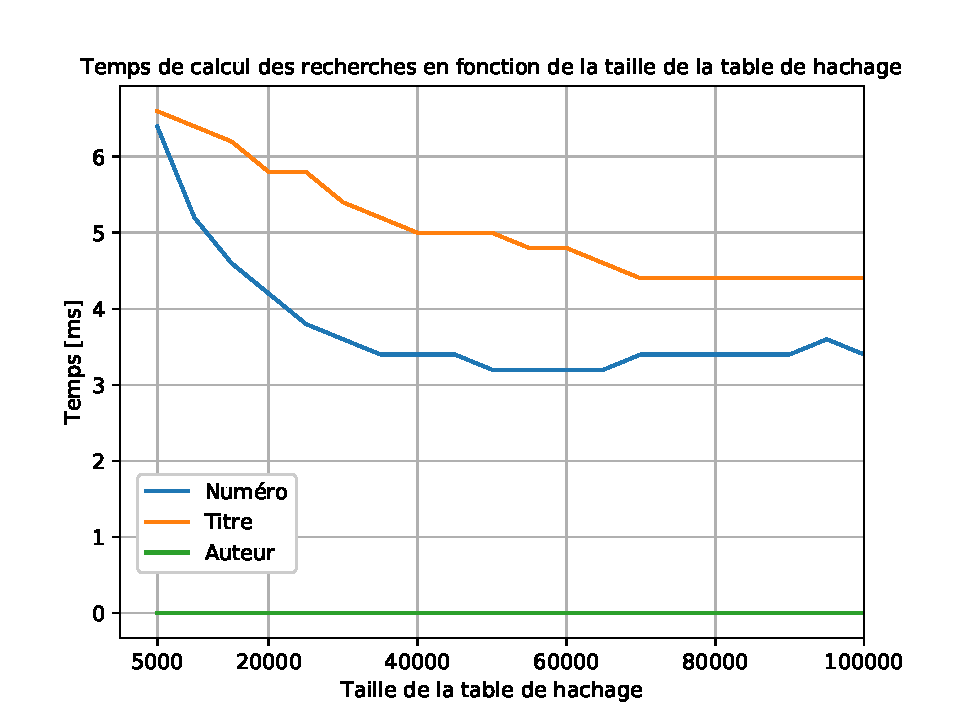
\includegraphics[scale=0.75]{FigQues3_2}
\caption{Temps d'exécution des recherches}
\label{FigQues32}
\end{figure}

On remarque que, comme décrit dans la question précédente, le temps de recherche par auteur ne change pas, restant à zéro pour toutes les valeurs de $m$. Pour les autres recherches, le temps de calcul décroit lorsque $m$ augmente, mais change très peu pour $m$ supérieur à 50~000. Une explication possible serait que, avec $m = 50 000$, on a en moyenne 2 éléments par entrée de la table de hachage, ce qui est déjà très petit, et donc on ne s'attend pas à d'importantes améliorations en augmentant le $m$. Cela justifie aussi notre choix de $m$ à la question précédente.

\section*{Question 3.3}

\begin{figure}[ht]
\centering
\begin{tabular}{@{} c @{} c @{}}
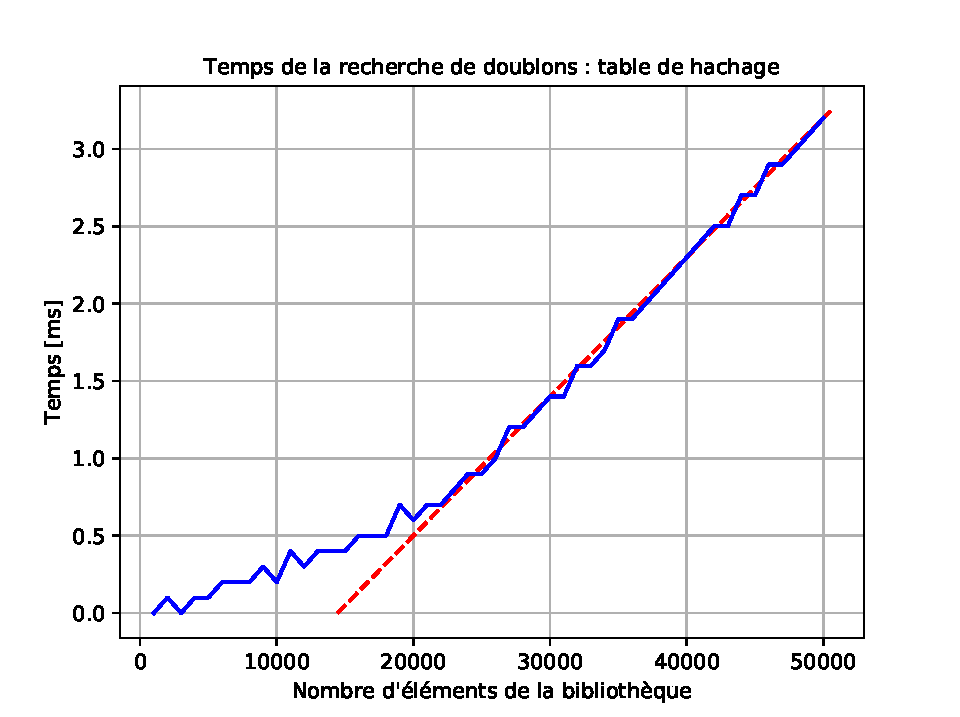
\includegraphics[width=0.5\textwidth]{FigQues3_3_hach_1} & 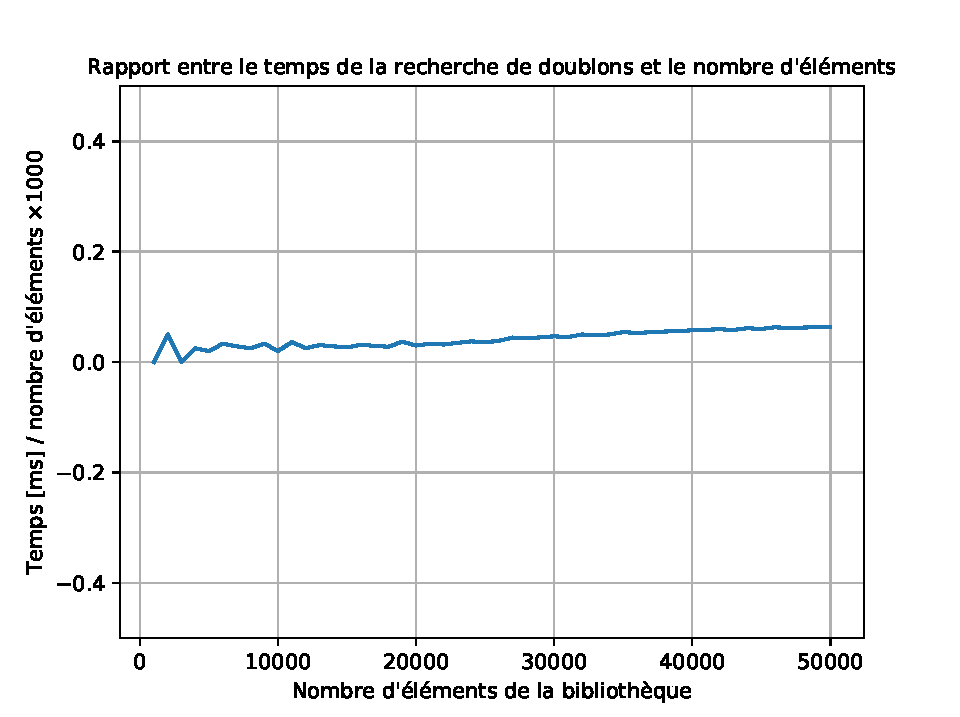
\includegraphics[width=0.5\textwidth]{FigQues3_3_hach_2} \tabularnewline
(a) & (b) \tabularnewline
\end{tabular}
\caption{Temps de recherche de doublons pour la table de hachage}
\label{FigQues3_3_hach}
\end{figure}

\begin{figure}[ht]
\centering
\begin{tabular}{@{} c @{} c @{}}
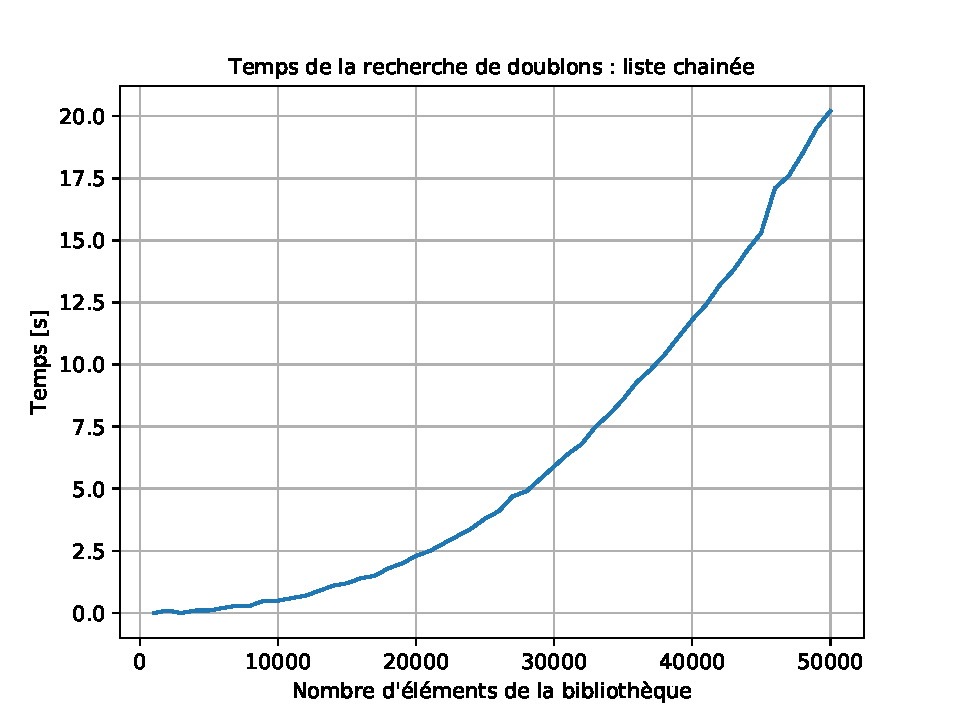
\includegraphics[width=0.5\textwidth]{FigQues3_3_list_1} & 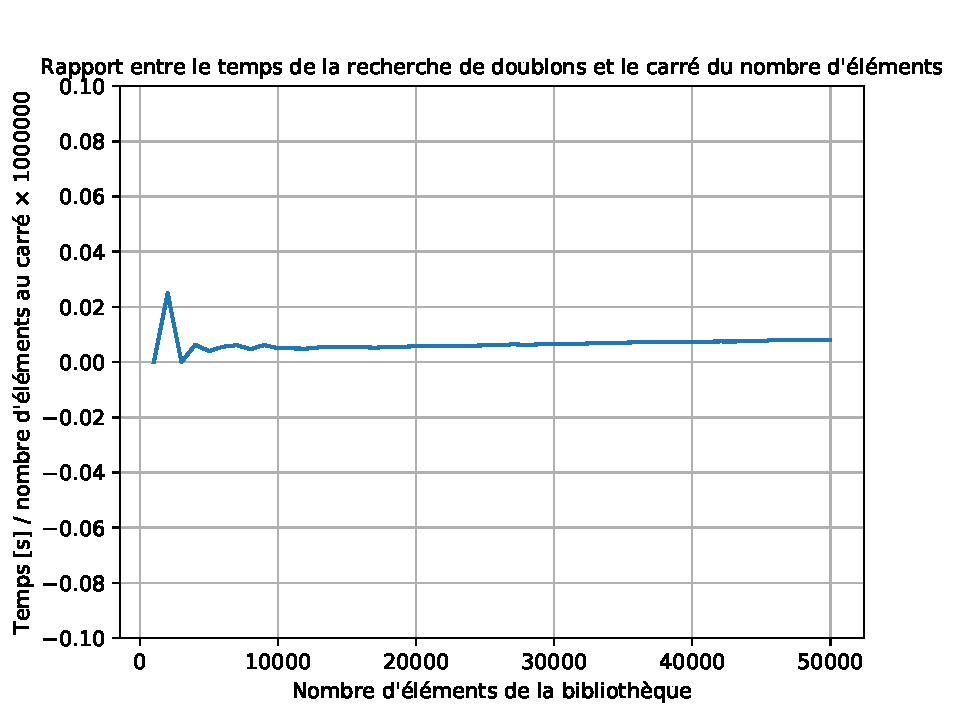
\includegraphics[width=0.5\textwidth]{FigQues3_3_list_2} \tabularnewline
(a) & (b) \tabularnewline
\end{tabular}
\caption{Temps de recherche de doublons pour la liste chainée}
\label{FigQues3_3_list}
\end{figure}

Les temps de recherche des ouvrages en doublons pour la table de hachage et la liste chainée sont donnés dans les Figures \ref{FigQues3_3_hach}(a) et \ref{FigQues3_3_list}(a), respectivement. Dans le cas de la Figure \ref{FigQues3_3_hach}, chaque temps a été calculé comme une moyenne de 10 000 simulations, alors que, pour la Figure \ref{FigQues3_3_list}, on a fait une moyenne de 10 simulations seulement. Nous attirons l'attention au fait que l'échelle verticale n'est pas la même pour les deux figures.

On remarque que, pour la table de hachage, à part pour quelques valeurs petites de nombre d'éléments, le comportement du temps de calcul est essentiellement linéaire. Pour mettre en évidence ce comportement, nous avons tracé, dans la Figure \ref{FigQues3_3_hach}(a), la droite qui coïncide avec les données expérimentales pour $n = 30000$ et $n = 50000$, et l'on observe que le comportement expérimental est très proche de cette droite pour $n \geq 20000$. Nous avons aussi tracé, dans la Figure \ref{FigQues3_3_hach}(b), le temps de calcul divisé par le nombre d'éléments, afin de vérifier que cette quantité est proche d'une constante.

Pour la liste chainée, le comportement du temps de calcul est quadratique, ce qui a été mis en évidence par la Figure \ref{FigQues3_3_list}(b), où nous avons tracé le temps de calcul divisé par le carré du nombre d'éléments, afin de vérifier que cette quantité est aussi proche d'une constante.

\section*{Question 3.4}

Dans le cas de la recherche de doublons avec une liste chainée, pour chaque élément de la liste, la fonction parcourt toute la liste une fois dans le pire des cas, où elle ne trouve pas de doublon pour cet élément. Ainsi, comme il faut répéter cette boucle pour chaque élément de la liste, la complexité est en $\Theta(n^2)$ au pire cas, où il n'y a pas de doublons dans la liste.

Dans le cas de la recherche de doublons avec une table de hachage de taille $m$ à $n$ éléments, on sait que tous les doublons seront forcément dans la même liste chainée, car ils auront la même clef. Alors la complexité est en $\Theta\left(m \left(\frac{n}{m}\right)^2\right)$, car, pour chacune des $m$ listes chainées, pour chacun de ses éléments, on parcourt toute cette liste à la recherche de ses doublons, et la taille moyenne d'une liste chainée est $\frac{n}{m}$.

Dans la Question 3.3, nous avons toujours choisi $m = \frac{n}{2}$, ainsi la complexité avec une table de hachage est en $\Theta\left(\frac{n}{2}\left(\frac{n}{n/2}\right)^2\right) = \Theta(2n) = \Theta(n)$.

\end{document}
